\chapter{Speech Emotion Recognition Using Acoustic Features}
\chaptermark{SER using acoustic features}

% \section{Introduction}
The purpose of this chapter is three-fold: (1) to investigate the effective
region of analysis for acoustic feature extraction, whether frame-based region
(local features) or utterance-based region (global features); (2) to evaluate
which action is the best with regard to the silence region in a dimensional
speech emotion recognition (SER); and (3) to evaluate which aggregation method
performs better for dimensional SER: acoustic input aggregation or output
aggregation (e.g., majority voting method). 

\section{Which region of analysis to extract acoustic features in SER}
\sectionmark{Region of Analysis}
\subsection{SER using low-level acoustic features}
% introduce frame-based processing
SER in conventional ways are performed by extracting acoustic features on
frame-based processing and then applied these features to a classifier. Let
$y(n)$, with $ n = 1, 2, 3, \ldots , L$, denotes acoustic signal with length
$L$.  In frame-based processing, this $y(n)$ signal is divided into many frames
by a fixed length. A typical length for a single frame is 16-25 milliseconds
(ms) with 10 ms to 15 ms hop length (stride). For 25 ms frame length and 10 ms
hop length, which is equal to 60\% overlap (15 ms), a window is applied to this
frame to make the short-time signal behave as a quasistationary signal -- near
the stationary signal. In their original length, an acoustic signal varies with
the time: non-stationary property.  Windowing processes the acoustic signal in
a short-term interval to remove this property. Figure
\ref{fig:frame-processing} shows the windowing process; short-term windowed
signals look stationary more than the original signal.

% # Windowing: why 25 ms, add figure, why overlapping

Windowing multiplies the spectrum of an input signal with window signal $w(n)$.
A typical window function for an acoustic signal is Hann and Hamming windows
(named after Julius von Hann and Richard W. Hamming).  The others are
rectangular, Bartlet, Kaiser, and Blackman.  The choice of the window function
is based on two aspects: the width of the main lobe and the additional lobes.
Hann and Hamming windows only differ in weighting factors with similar concept:
cosine-sum windows

\begin{equation}
  w[n] = A + B \cos \biggl(\frac {2\pi n}{M}\biggl), ~~~~~n = -M/2, \ldots, M/2,
\end{equation}

\noindent where $A$ is $0.5$ for Hann and $0.54$ for Hamming. $B$ is $0.5$ for
Hann and $0.46$ for Hamming. Both window functions are widely used in speech
processing due to a good trade-off between time and frequency resolution
(effect of side lobes). Figure \ref{fig:window_hann} shows a Hann window and
its spectrum, while Figure \ref{fig:windowing_demo} shows an example of a
Hamming window applied to a sinusoid signal and its result.

\begin{figure}[htbp]
  \centering
  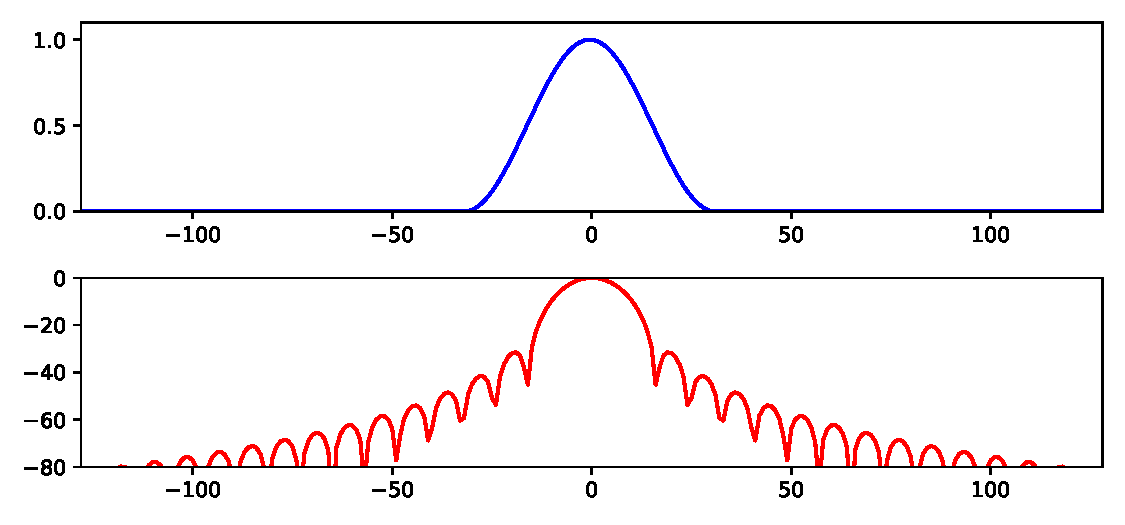
\includegraphics[width=\textwidth]{../fig/window_hann.pdf}
  \caption{Hann window and its spectrum}
  \label{fig:window_hann}
\end{figure}

\begin{figure}[htbp]
  \centering
  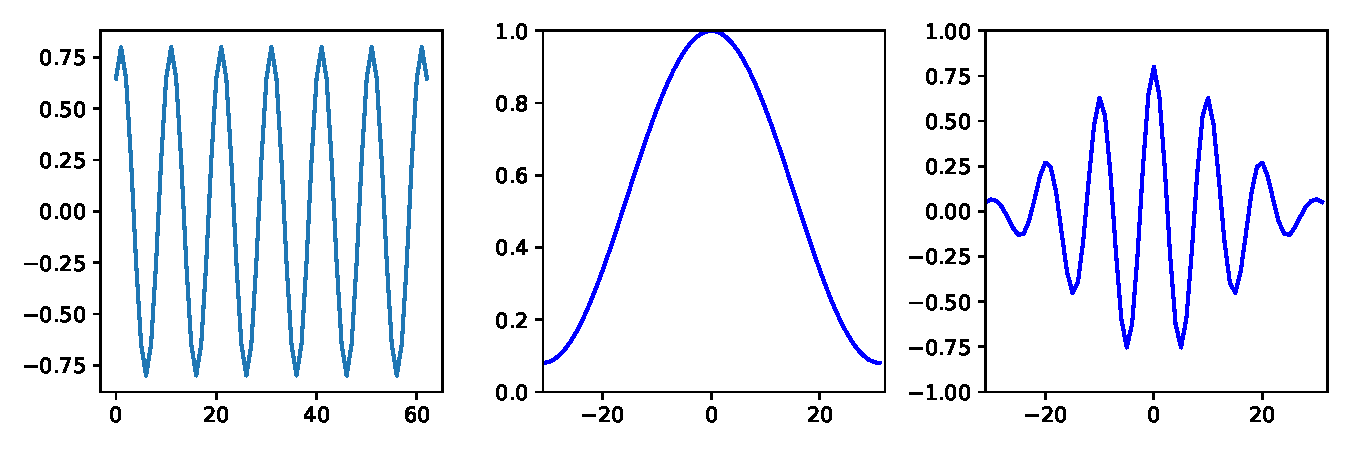
\includegraphics[width=\textwidth]{../fig/windowing_demo.pdf}
  \caption{An example of Hamming window (middle) applied to sinusoid signal (left); the resulted windowed signal (right) is multiplication of both.}
  \label{fig:windowing_demo}

\end{figure}
The length of a window is usually equal to the length of the frame: one window
per frame. If the length of a window is smaller than a frame, each frame will
be windowed with window length and padded with zeros to match the frame's
length. In speech emotion recognition, a short window is used to capture short
dynamics context while a longer window is used to capture mid and longer
dynamics. A common approach used a short window to extract acoustic features in
short-term time while statistical functions model long-term dynamics. Figure
\ref{fig:frame-processing} shows the frame-based processing of an acoustic
signal (speech), which windows short-term signals using the Hamming window.

\begin{figure}[htbp]
  \centering
  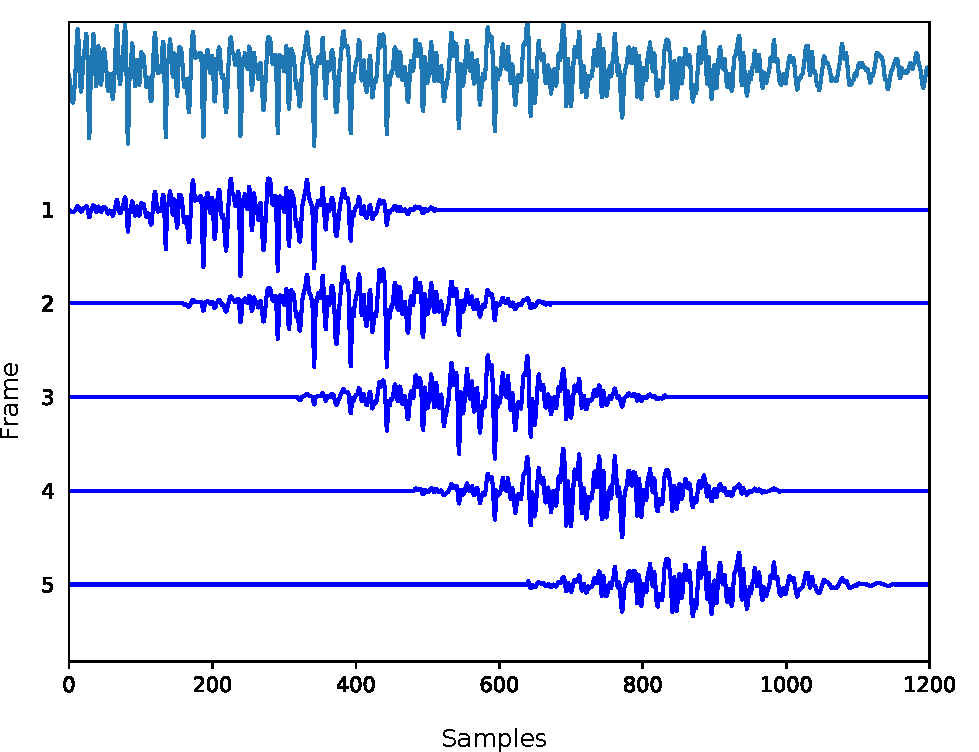
\includegraphics[width=\textwidth]{../fig/framing.pdf}  
  \caption{Frame-based processing for extracting low-level descriptors of an acoustic signal; the signal is an excerpt of IEMOCAP utterance with 400 samples frame length and 160 samples hop length; sampling frequency is 16 kHz.}
  \label{fig:frame-processing}
\end{figure}

% # LLD, MFCC, Why
The acoustic features extracted from each frame are known as local features or
low-level descriptors (LLD) \cite{Herrera1999}. The most common LLD for speech
processing is mel-frequency cepstral coefficients (MFCC). MFCC captures
different aspects of the spectral shape of a speech. The following steps
compute MFCC in sequences. First, FFT/DFT transformed a time-domain signal into
a frequency domain signal (spectra). Second, the mel frequency warping function
converts spectra in linear scale into the mel scale. Although several functions
have been proposed, a common approach keeps linear scale for acoustic
frequencies below 1 kHz and converts to logarithmic scale for acoustic
frequencies above 1 kHz. This conversion imitates the human perceptual system.
Third, convert a power spectrogram (amplitude squared) to decibel (dB) units
($\log$). Finally, DCT computes MFCC as amplitude cepstra.

% number of mfcc coefficients; the number of frames; the shape of MFCC
One of the important parameters in MFCC is the number of coefficients. A number
of 13 to 40 coefficients are common for speech processing. For each frame, 13
MFCCs are extracted. If there are 40 frames in an utterance, the dimension of
MFCC features will be (40, 13). The number of frames corresponds to the number
of samples divided by hop length (in samples).  If an utterance comprises 1
second (s) with a 16 kHz sampling rate, the number of samples is 16000. Using
25 ms (400 samples) window/frame length and 10 ms (160 samples) hop length, the
number of frames is $16000/160$, i.e., 100 frames. Figure \ref{fig:mfcc-mel}
top shows an MFCC spectrogram of an IEMOCAP utterance with 13 coefficients.

% mel-spectrogram and log mel-spectrogram
Recently, researchers found that mel-spectrogram, also called as (mel)
filterbank or mel-frequency spectral coefficients (MFSC), yields better
performance for deep learning-based automatic speech recognition (ASR) (e.g.,
\cite{Mohamed2014}). Given that a deep learning system is less susceptible to
highly correlated input, the DCT step in the previous MFCC calculation is not
necessary since it is a linear transformation.  DCT discards some information
in speech signals, which are highly non-linear \cite{fayek2016}. Furthermore, a
log version (in decibel unit) of mel-spectrogram, i.e., log mel-spectrogram, is
preferable since deep learning learns better in this unit. The conversion from
mel-spectrogram to log mel-spectrogram is given by

\begin{equation}
  S_{dB} = 10 \log \biggl( \frac {S}{ref}\biggr),
  \label{eq:log-mel}
\end{equation}
\noindent where $S$ is the input power spectrogram and $ref$ is reference
power. A value of $1.0$ is a common $ref$ value for 32-bit floating-point data
type (`float32').

% show and interpret figure
Figure \ref{fig:mfcc-mel} shows the visualization of MFCC, mel-spectrogram and
log mel-spectrogram. From this figure, it is clear that the log mel-spectrogram
is more informative than the mel-spectrogram and MFCC. This visualization may
support the previous argument that log mel-spectrogram may works better in
DNN-based speech emotion recognition.

\begin{figure}[htbp]
  \centering
  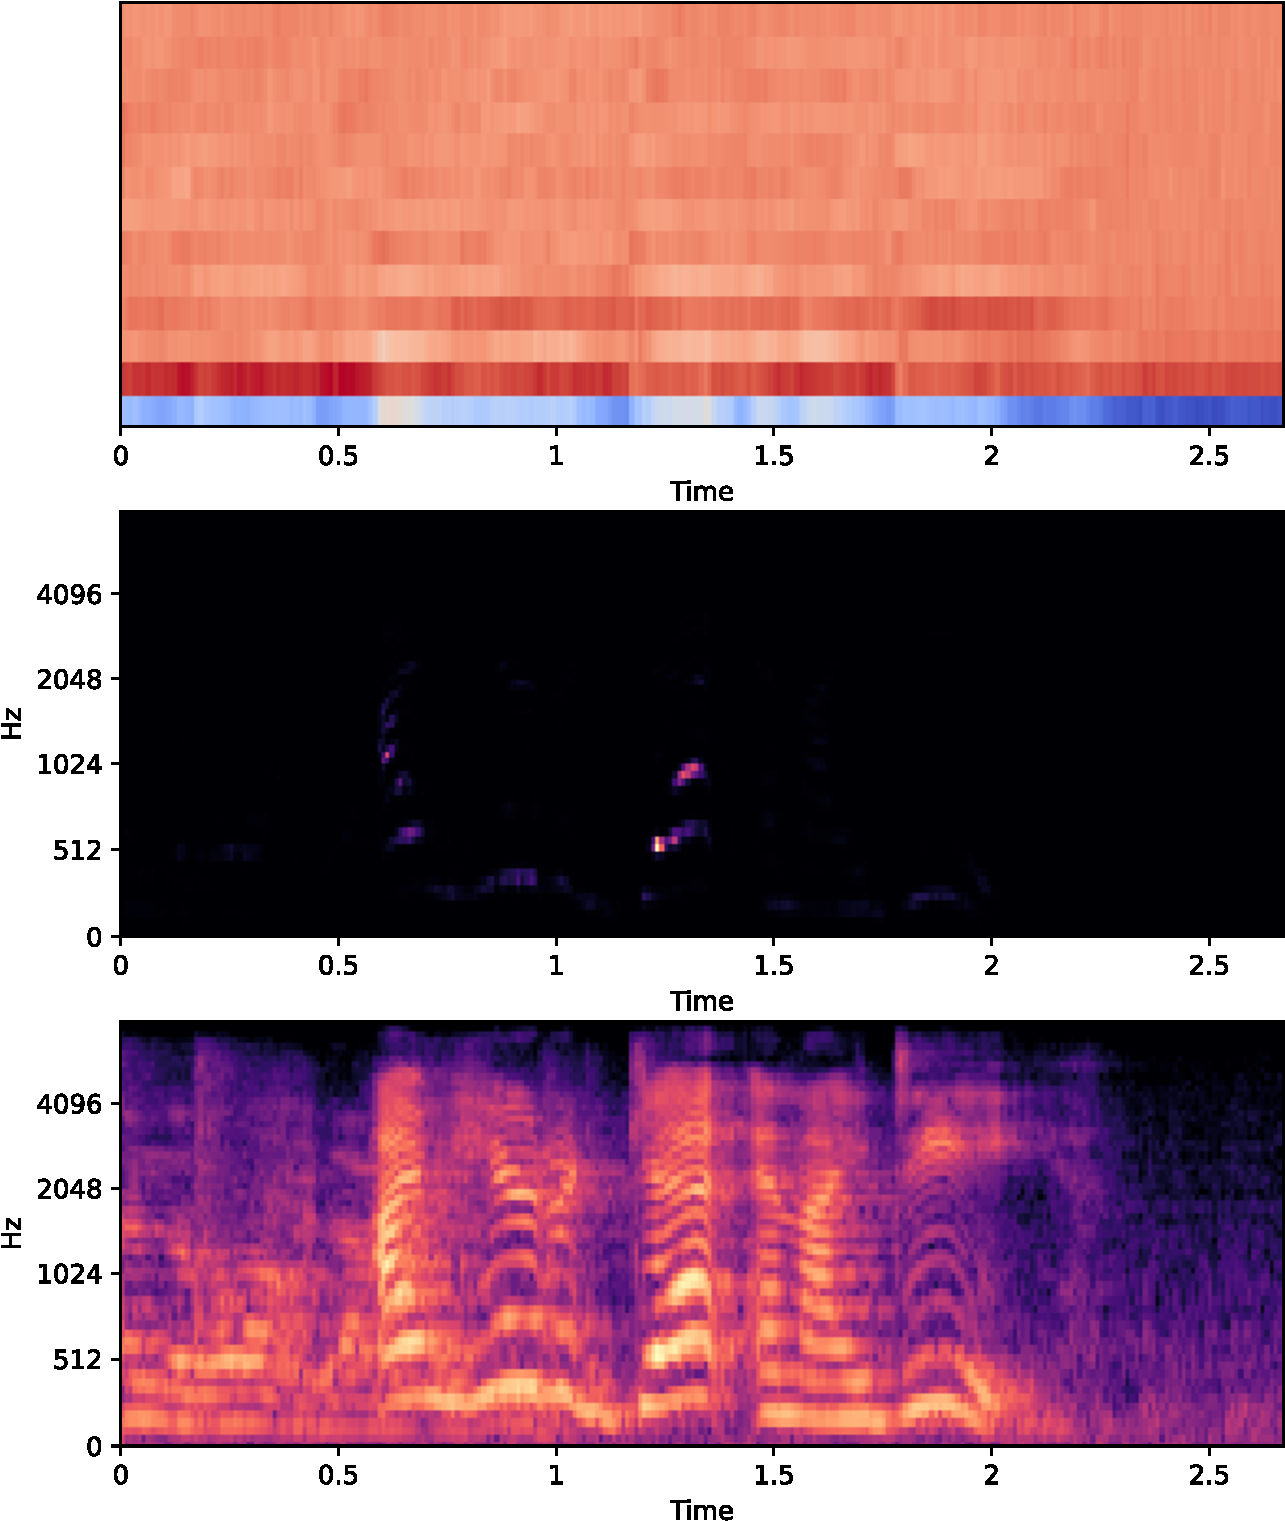
\includegraphics[width=.7\textwidth]{../fig/mfcc-mel-crop.pdf}
\caption{Visualization of MFCC features with 13 coefficients (top),
mel-spectrogram (middle), and log mel-spectrogram with 64 mels (bottom)}
  \label{fig:mfcc-mel}
\end{figure}

Apart from the use of one type of acoustic features for speech processing, some
researchers have proposed a set of acoustic features for speech emotion
recognition. Eyben et al. \cite{Eyben} proposed Geneva minimalistic parameter
set (GeMAPS) as a standard acoustic feature set for affective voice research.
The proposed acoustic features are based on (1) physiological changes in voice
production, (2) proven significance in previous studies, and (3) theoretical
significance. The proposed acoustic feature set comprises 23 LLDs, as shown in
Table \ref{tab:gemaps_paa}. This acoustic feature set is extracted on a frame
processing basis with 25 ms frame length and 10 ms hop length.

% pyAudioanalysis
Giannakopoulos \cite{Giannakopoulos2015} proposed pyAudioanalysis as an
open-source Python library for audio signal analysis. The library supports a
wide range of audio analysis procedures such as feature extraction,
classification, supervised and unsupervised segmentation, and visualization.
Different from GeMAPS feature set, pyAudioanalysis targets a wide range of
voice applications like audio event detection, speech emotion recognition,
music segmentation, and health application. The short-term feature set, which
is extracted on a frame-based processing, consists of 34 LLDs. These LLDs are
shown in Table \ref{tab:gemaps_paa}.

\begin{table}[htpb]
\caption{Acoustic feature sets: GeMAPS \cite{Eyben} and pyAudioAnalysis
\cite{Giannakopoulos2015}. The numbers in parentheses indicate the total
numbers of features (LLDs).}
\label{tab:gemaps_paa}
  \begin{center}
\begin{tabular}{p{7.5cm} | p{7cm}}
  \hline 
\hspace{2.5cm}GeMAPs (23) & \hspace{1.5cm}pyAudioAnalysis (34) \\
\hline \hline
intensity, alpha ratio, Hammarberg index, spectral slope 0-500 Hz, spectral
slope 500-1500 Hz, spectral flux, 4 MFCCs, $f_o$, jitter, shimmer,
harmonics-to-noise ratio (HNR), harmonic difference H1-H2, harmonic difference
H1-A3, F1, F1 bandwidth, F1 amplitude, F2, F2 amplitude, F3, and F3 amplitude.
& zero crossing rate, energy, entropy of energy, spectral centroid, spectral
spread, spectral entropy, spectral flux, spectral roll-off, 13 MFCCs, 12 chroma
vectors, chroma deviation.\\
  \hline 
  \end{tabular}
\end{center}
 \end{table}

% Result
As additional features sets, a temporal difference on pyAudioAnalysis were
computed in the first order, referred to \emph{deltas}. The addition of the
first-order regression coefficients shows better performances than original LLDs
(MFCC and MFSC) in ASR. In dimensional SER, these temporal differences may show
the dynamics between frames. Together with the previous four feature sets,
these LDDs are compared to evaluate the effectiveness of frame-based LLDs in
dimensional SER. 

% interpret table
Table \ref{tab:iemocap-lld} shows the performance of dimensional SER from
IEMOCAP dataset in CCC scores. There is no remarkable difference in the use of
different common acoustic features used in acoustic signal processing. This
presented results also challenged the specially designed acoustic features
namely GeMAPS \cite{Busso2008} which is proposed to be the standard feature set
for voice research and affective computing \cite{Eyben}. Although it achieves
the highest score in LLD comparison, the general-purpose pyAudioAnalysis (pAA)
features set attained a comparable performance to GeMAPS, and in later analysis
it will be shown that this feature set achieve a higher performance than GeMAPS
on utterance-based feature extraction. 

\begin{table}
    \caption{Results of frame-based LLDs for dimensional SER in IEMOCAP dataset}
    \begin{center}
    \begin{tabular}{l | c | c c c c}
      \hline 
Feature & Dim & Val & Aro & Dom & Mean \\
\hline \hline
MFCC      & (3414, 40)    &0.148    & 0.488   & 0.419   & 0.352 \\
Log mel   & (3414, 128)   &0.103    & 0.543   & 0.438   & 0.362 \\
GeMAPS    & (3409, 23)    &0.164    & 0.527   & 0.454   & 0.382 \\
pAA       & (3412, 34)    &0.130    & 0.513   & 0.419   & 0.354 \\
pAA\_D    & (3412, 68)    &0.145    & 0.526   & 0.439   & 0.370 \\
      \hline
    \end{tabular}
    \label{tab:iemocap-lld}
  \end{center}
\end{table}



% Summary LLD and Problem with frame-based processing: high-dimensions, needs
% zero padding

\subsection{SER using high-level acoustic features}
% GeMAPS
In the previous subsection, it is shown that frame-based acoustic features work
with limited performance. In this subsection, the effectiveness of the two
statistical functions is shown. Two high-level acoustic features, i.e., mean
values and standard deviations from LLDs, are evaluated from the previous five
acoustic feature sets. 

% describe mean
The first high-level acoustic features used for this dimensional SER task are
mean values. The idea of using these mean values is to capture the shared
information across all frames. This arithmetic mean values can be formulated
as: 

\begin{equation}
  \mu_F = \frac{1}{\mathcal{K}}\sum _{i=1}^\mathcal{K} F_i  
\end{equation}

\noindent where $\mathcal{K}$ is the number of frames,  and $i$ is the frames'
index, and $F$ is the corresponding feature.  For instance, in pyAudioAnalysis,
the first feature is a zero-crossing rate (ZCR).  The ZCR feature's mean value
is the arithmetical mean of all ZCR values in all frames within an utterance.  

% describe std
The second high-level acoustic features are standard deviation (std). This
statistical function shows the dispersion of feature values from its mean.
While mean is intended to capture the commonalities among features values in
all frames within an utterance, std is intended to capture the dynamics of
feature values in an utterance. Accordingly, std is formulated as follows, 

\begin{equation}
  \sigma_F^2 = \frac{1}{\mathcal{K}}\sum _{i=1}^\mathcal{K} (F_i - \mu_F)^2.
\end{equation}

% recap mean+std
Both mean and std (Mean+Std) are known as valuable functions in SER.
References \cite{Sebastian2019, Morales2016, Tomas2019} have used Mean+Std for
categorical SER. However, most references did not use only Mean+Std, but other
statistical functions like median, quartiles, minimum, maximum, and other
features. It is interesting to experiment with Mean+Std only for dimensional
SER given the fact that both high-level features are two most informative
descriptors, among other statistical functions. Besides reducing the size or
dimension of features significantly, using Mean+Std consequently speed up the
computation of SER with regard to their small input features.

Another advantage of using Mean+Std features is no need for zero paddings.
Although zero paddings are useful for FFT calculation (spectral smoothness), it
is unclear the effect of zero paddings on LLDs for acoustic feature extraction.
Zero padded values may impact information represented by features when such
processing is performed, e.g., standardization or normalization. Hence,
acoustic features represented by Mean+Std features are more informative than
LLDs since it only contains information from speech. 

An illustration of Mean+Std extraction from LLDs is shown in Figure
\ref{fig:mean_std}. For instance, an MFCC feature set from an utterance
consists of 3414 frames with 40 MFCC coefficients. For each mean and std
features, 40 values are calculated. Both mean and std are concatenated to form
Mean+Std features after transposing both statistical features.

\begin{figure}[htbp]
  \centering
  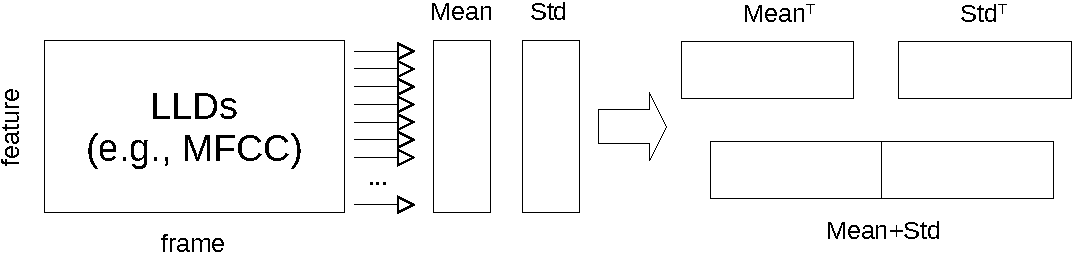
\includegraphics[width=0.9\textwidth]{../fig/mean_std-crop.pdf}
  \caption{Illustration of Mean+Std extraction from LLDs (e.g., MFCCs)}
  \label{fig:mean_std}
\end{figure}

% shows result

\begin{table}
    \caption{Results of utterance-based HSF for dimensional SER in IEMOCAP dataset}
    \begin{center}
    \begin{tabular}{l | c | c c c c}
      % \hline
      \hline
Feature & Dim & Val & Aro & Dom & Mean \\
\hline \hline
MFCC      &   80  & 0.155 & 0.580   & 0.456 & 0.397 \\
Log Mel   &   256 & 0.151 & 0.549   & 0.455 & 0.385 \\
GeMAPS    &   46  & 0.191 & 0.523   & 0.452 & 0.389 \\
pAA       &   68  & 0.145 & 0.563   & 0.445 & 0.384 \\
pAA\_D     &  128  & 0.173 & 0.612   & 0.455 & 0.413 \\
      \hline
      % \hline
    \end{tabular}
    \label{tab:iemocap-hsf}
  \end{center}
\end{table}

% show and discuss pAA\_D obtain the best performance
\subsection{Optimizing dimensional SER using different classifiers}
% \section{Evaluation Metric} \section{Experiment and Results on Region
% Analysis of Acoustic Features}
In the previous subsections, the study focuses on the search for relevant
acoustic features (regions) for feature extraction. As described in the
previous chapter, two important components of SER are features and classifiers.
In this subsection, a study to optimize dimensional SER using different
classifiers is presented. 

Long short-term memory (LSTM) networks are used to obtain the previous results
on both LLDs and Mean+Std features. The LSTM network consists of 3 layers with
256 units each. This configuration is based on \cite{Atmaja2020d}. Since the
input is a sequence of acoustic features, using a recurrent-based LSTM network
is a straightforward approach. The use of LSTM as a classifier for SER has been
found useful for both dimensional \cite{Schmitt2018} and categorical task
\cite{Atmaja2019}. While the previous results used three layers with the same
units, this optimization section varies one to five layers with a different
number of units.

Apart from LSTM networks, convolutional neural networks (CNN) and multilayer
perceptrons (MLP) were accommodated. Both CNN and MLP use varying layers and
their corresponding units, as shown in Table \ref{tab:layer}. CNN has been
found to be useful for image-like input. Log mel-spectrogram is an example of
this input. MLP, one of the oldest neural network architecture, remains useful
due to its simplicity to model complex internal representation of their
environment \cite{Hinton1989}. While the implementation of both LSTM and CNN
were performed by using Keras toolkit \cite{chollet2015keras}, the
implementation of MLP was performed using the scikit-learn toolkit
\cite{scikit-learn}.

\begin{table}
  \caption{Number of layer and corresponding units on each layer}
  \begin{center}
      \begin{tabular}{c  c}
          \hline
\# layers   &   \# units \\
\hline \hline
1   &   (16) \\
2   &   (32, 16) \\
3   &   (64, 32, 16) \\
4   &   (128, 64, 32, 16) \\
5   &   (256, 128, 64, 32, 16) \\
6   &   (512, 256, 128, 64, 32, 16) \\
          \hline
      \end{tabular}
      \label{tab:layer}
  \end{center}
\end{table} 

% interpret table
Table \ref{tab:iemocap-optim} and \ref{tab:improv-optim} show results of
optimizing dimensional SER using different classifiers from IEMOCAP and
MSP-IMPROV datasets. As for the input, all networks take the previous
pyAudioAnalysis with deltas (pAA\_D). Changing the number of layers and their
units changes their performances, as well as changing the classifiers. Using
CNN, an improvement from the previous LSTM result was obtained with a single
layer with 16 nodes. On using MLP, significant improvements were obtained; the
highest average CCC score was obtained using five layers for IEMOCAP and four
layers for MSP-IMPROV. The average CCC score of this architecture is 0.472 for
IEMOCAP and 0.433 for MSP-IMPROV. These high results should be evaluated in the
same framework (toolkit) in the future; this study evaluated LSTM and CNN using
Keras with TensorFlow back-end while MLP is performed using scikit-learn
toolkit.

\begin{table} [!htbp]
\caption{Average CCC score on IEMOCAP dataset using different classifiers and
number of layers (features: pAA\_D)}
    \begin{center}
    \begin{tabular}{l | c c c c c c}
      \hline 
Classifier &   1lay & 2lay  & 3lay  & 4lay  & 5lay  & 6lay  \\
\hline \hline
LSTM  & 0.389 & 0.403 & 0.385 & 0.401 & 0.395 & 0.399 \\
CNN   & 0.415 & 0.399 & 0.380 & 0.376 & 0.390 & 0.379 \\
MLP   & 0.450 & 0.469 & 0.448 & 0.462 & 0.472 & 0.452 \\
      \hline
    \end{tabular}
    \label{tab:iemocap-optim}
  \end{center}
\end{table}

\begin{table}[!htbp]
\caption{Average CCC score on MSP-IMPROV dataset using different classifiers
and number of layers (features: pAA\_D)}
  \begin{center}
  \begin{tabular}{l | c c c c c c}
    \hline 
Classifier &   1lay & 2lay  & 3lay  & 4lay  & 5lay  & 6lay  \\
\hline \hline
LSTM & 0.350  & 0.378 & 0.372 & 0.343 & 0.317 & 0.354 \\
CNN  & 0.356  & 0.335 & 0.326 & 0.349 & 0.382 & 0.296 \\
MLP  & 0.413  & 0.420 & 0.421 & 0.433 & 0.359 & 0.369 \\
    \hline
  \end{tabular}
  \label{tab:improv-optim}
\end{center}
\end{table}

% show and discuss why MLP obtain the best
To this end, several steps to observe which region of analysis to extract
acoustic features were performed. At first, the common LLDs, like MFCC
features, were evaluated. Later, the Mean+Std of these LLDs were used as input
features to the same classifier. The results clearly show that extracting
statistical functions over frame-based LLDs is better. Mean+Std with small size
($80$ vs. ($3414 \times 40$)) consistently performs better than LLDs. An
optimization using different classifiers shows improvements from the previous
LSTM networks with the same high-level acoustic features. 

\section{Effect of silent pause features in dimensional SER}
In the previous section, analysis of region for acoustic feature extraction was
investigated. This section investigates the second issue in dimensional SER
using acoustic features: which action is better to treat silent pause region in
dimensional SER. There are three actions that can be taken regarding silent
pause in SER:
\begin{itemize}
\item removing silence: extract acoustic features from speech-segment only,
\item keeping silence: extract acoustic features from the whole utterance,
including speech and silence regions,
\item utilizing silence: utilize silent pause regions as acoustic features.
\end{itemize}
The goal of this section is to examine which action from these three serves the
best for dimensional SER. The second action was already evaluated in the
previous results; therefore, only first and third actions will be explained and
evaluated in this section. The baseline uses pAA features (with 68 HSFs) to
observe the difference among the silence-removed region, silence-kept region,
and silent pause features as an additional feature.

% \subsection{Dimensional SER on silence-kept region}

\subsection{Dimensional SER on silence-removed region}
% add intro why silence could be important removing silence
Removing silence is a common practice in speech processing. ASR avoids
recording silent voice and only uses voiced speech to save power and
computational load. In automatic SER, the contribution of silence in speech is
not clear until now. Aguilar et al. \cite{Aguilar2020} evaluated both removing
and keeping silence for unimodal and multimodal categorical emotion
recognition. The result is different.  Keeping silences lead to better
performance in unimodal emotion recognition, while multimodal shows that
removing silence is better than keeping silence. Atmaja and Akagi
\cite{Atmaja2019} showed that removing silence leads to higher accuracies score
than using whole speech in categorical speech emotion recognition. 

% calculating RMS
A naive way to calculate silence region within speech is by using root mean
square (RMS) energy. Given a threshold $\tau$, if the RMS energy of a speech
frame below this $\tau$ threshold, then that frame is categorized as a silence.
The RMS energy is given by the following equation:
\begin{equation}
  x_{rms} = \sqrt{\dfrac{1}{n} (x_1^2 + x_2^2 + \ldots + x_n^2)}.
\end{equation}
As shown in Figure \ref{fig:silence} (b), a threshold of $0.065$ is a
reasonable choice for given speech utterance (an excerpt from IEMOCAP dataset).
However, this RMS energy curve occasionally fall below the threshold for a
moment and these values are not counted as silence. A better way to detect
silence is by probability mapping, a conversion from raw RMS energy to a
likelihood/probability. The probability mapping is formulated as 
\begin{equation}
  P[NS=1 | x_{rms}] = \frac{\exp(x_{rms} - \tau)}{1 + \exp(x_{rms} - \tau)}.
\end{equation}
The result is shown in Figure \ref{fig:silence} (c). The final part in the
bottom of the figure shows the result in binary value, an $NS$ of 1 for
non-silence and 0 for silence.

\begin{figure}
  \centering
  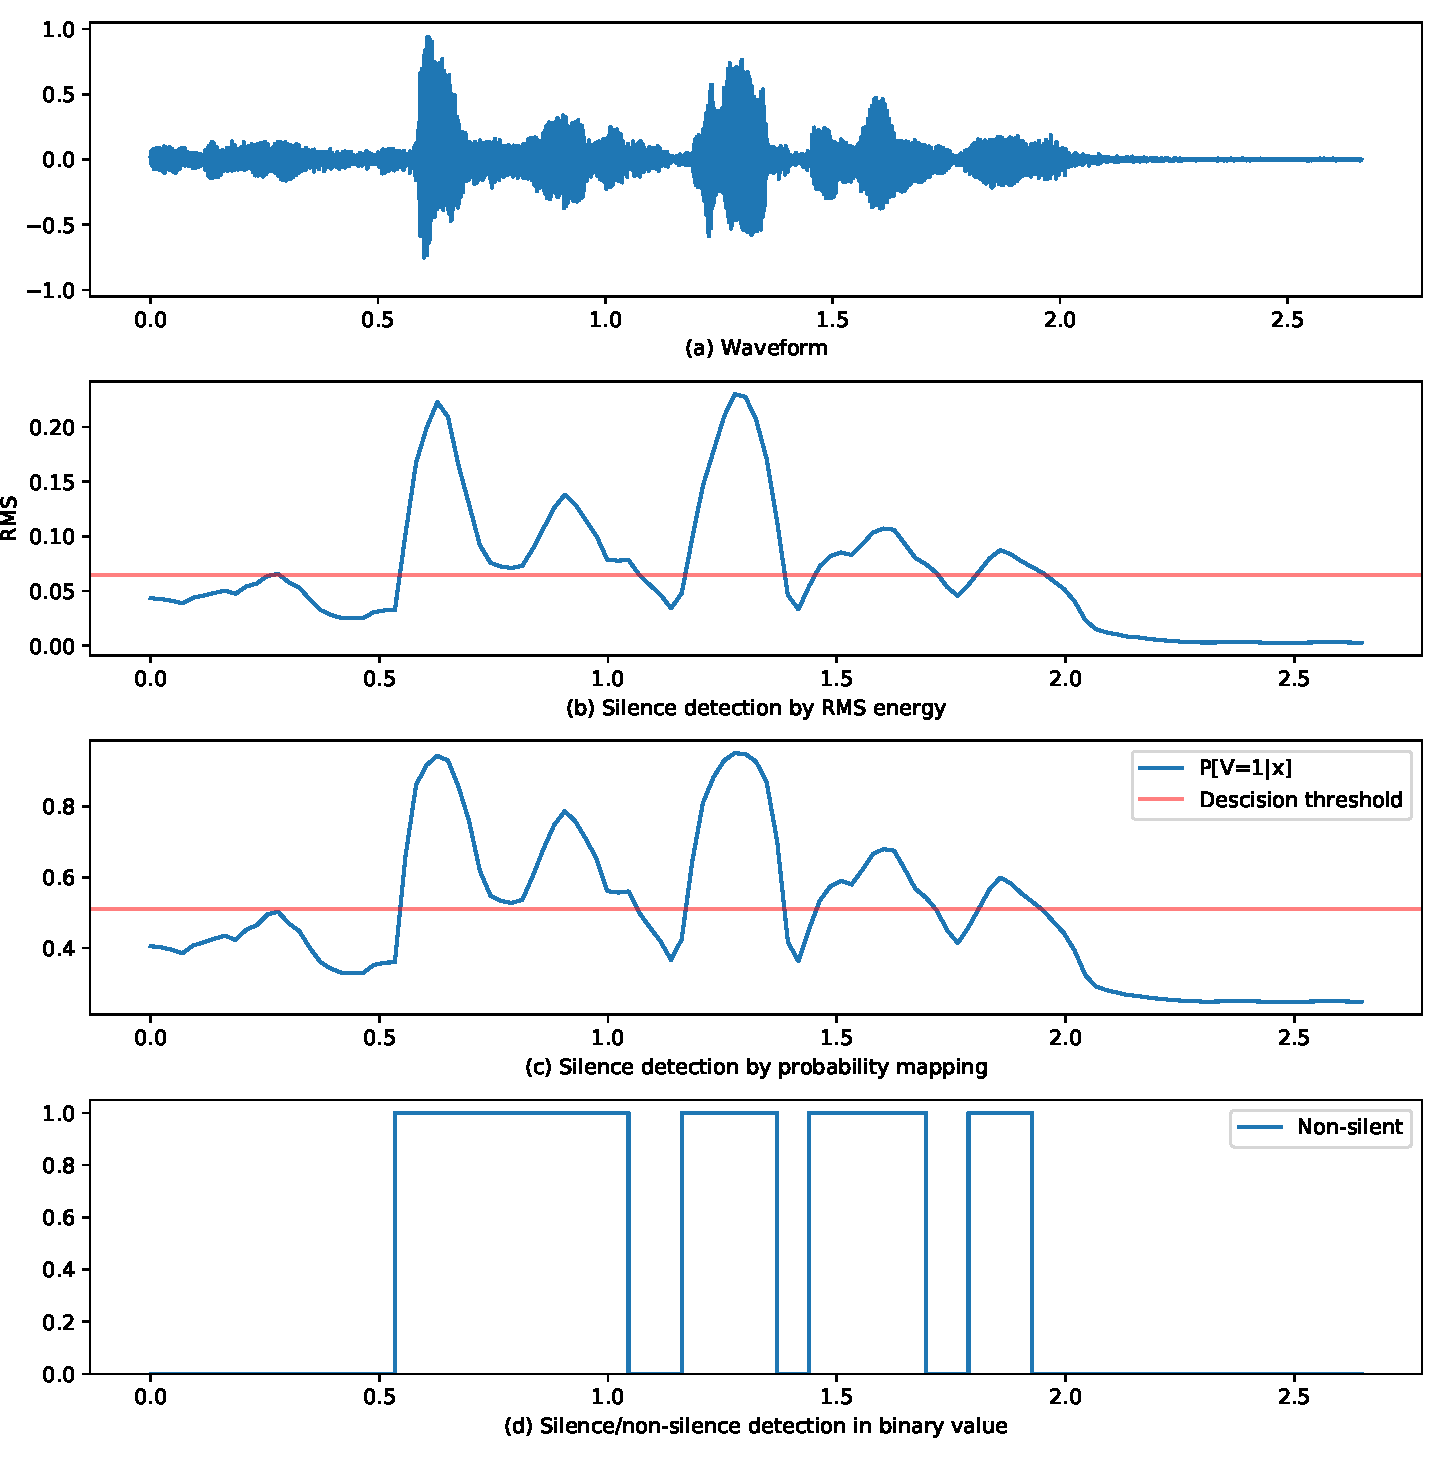
\includegraphics[width=\textwidth]{../fig/silence.pdf}
  \caption{Calculation of silent region in speech}
  \label{fig:silence}
\end{figure}

In practice, using a threshold $\tau$ as a percentage from maximum values is
more intuitive while it gives a similar result. Additionally, (minimum)
duration of silence is another important parameter. The minimum number of
samples to be removed represents the duration of the pause in speech
communication, which has been studied thoroughly \cite{Campione2002}. These two
parameters, silence $\tau$ and duration $d$, can be used to experiment with 
the removal of silence regions and to extract the acoustic features from these
regions.

Three different thresholds and durations were performed to remove silence from
the speech dataset. For the threshold, the values of 0.01\%, 0.1\%, and 5\%
were examined, while for durations were 10 ms, 60 ms, and 100 ms. The results
are shown in Table \ref{tab:sil_remove_ie}. As the baseline method, MLP with
Mean+Std of pyAudioAnalysis features (without deltas, 68 dimensions) were used.
The baseline method gains 0.458 of the average CCC score. Among nine
combinations of duration and threshold for removing silences where acoustic
features were extracted, only one result shows a higher performance than the
baseline. This result is in line with previous research (\cite{Atmaja2019,
Tian2015a, Aguilar2020,Fayek2017}), in which special adjustments are needed to
take the benefit of treating silent pause regions in speech.

\begin{table}
\caption{Result of using different duration and threshold factor for removing
silence on IEMOCAP dataset; bold-typed scores indicate a higher value than
baseline.}
  \begin{center}
  \begin{tabular}{c | c | c c c c}
    \hline
Duration (ms)   & Threshold (\%) &  V & A & D & Mean \\
\hline \hline
10  & 0.1 & 0.283 & 0.640 & 0.454 & \textbf{0.459} \\
10  & 1   & 0.234 & 0.560 & 0.418 & 0.404 \\
10  & 5   & 0.205 & 0.568 & 0.393 & 0.389 \\
60  & 0.1 & 0.279 & 0.625 & 0.453 & 0.452 \\
60  & 1   & 0.255 & 0.574 & 0.425 & 0.418 \\
60  & 5   & 0.209 & 0.567 & 0.398 & 0.391 \\
100 & 0.1 & 0.281 & 0.629 & 0.456 & 0.455 \\
100 & 1   & 0.276 & 0.571 & 0.429 & 0.425 \\
100 & 5   & 0.205 & 0.557 & 0.393 & 0.385 \\
    \hline
  \end{tabular}
  \label{tab:sil_remove_ie}
  \end{center}
\end{table}


\begin{table}
\caption{Result of using different duration and threshold factor for removing
silence on MSP-IMPROV dataset; bold-typed scores indicate a higher value than
baseline.}
  \begin{center}
  \begin{tabular}{c | c | c c c c}
    \hline
Duration (ms)   & Threshold (\%) &  V & A & D & Mean \\
\hline \hline
10  & 0.1  & 0.228  & 0.575   & 0.437   & \textbf{0.413} \\
10  & 1    & 0.246  & 0.581   & 0.431   & \textbf{0.420} \\
10  & 5    & 0.148  & 0.569   & 0.414   & 0.377 \\
60  & 0.1  & 0.241  & 0.588   & 0.442   & \textbf{0.424} \\
60  & 1    & 0.259  & 0.586   & 0.441   & \textbf{0.429} \\
60  & 5    & 0.184  & 0.569   & 0.415   & 0.389 \\
100 & 0.1  & 0.239  & 0.587   & 0.438   & \textbf{0.421} \\
100 & 1    & 0.252  & 0.580   & 0.430   & \textbf{0.421} \\
100 & 5    & 0.201  & 0.574   & 0.422   & 0.399 \\
    \hline
  \end{tabular}
  \label{tab:sil_remove_msp}
  \end{center}
\end{table}

\subsection{Dimensional SER with silent pause features}
% other research that say silence is useful for emotion
Tian et al. \cite{Tian2015a} argued that silence is an effective cue for
recognizing emotion.  Using this idea, Fayek et al. \cite{Fayek2017} used
silence as an additional category for detecting emotion categories from the
speech signal. Silent pause length also plays an important role in ascribing
emotions based on psychoacoustics experiment \cite{Tisljar-Szabo2014}. These
assumptions along with their results are motivations to use silence as a
feature for dimensional SER.

There are several ways to count silent pause features in speech. A
straightforward way is by detecting the number of silent regions and compared
them to the whole utterance. The result is a portion of silence region over
speech. Although this method may represent silent pause more precisely, there
is more effort needed to align the timing of spoken words and silence region
manually to obtain a more accurate result. Alternatively, silent pause
detection can be done on frame basis calculation with fixed-length samples (of
speech signals). A frame, then, can be categorized as silence or non-silence by
a specific rule.

A silent pause feature, in this research, is defined as the proportion of
silent frames among all frames in an utterance. In human communication, the
proportion of silence in speaking depends on the speaker's emotion. For
example, a happy speaker may have fewer silences (or pauses) than a sad
speaker. The proportion of silence in an utterance can be calculated as

\begin{equation}
  \label{eq:sil_ratio}
  sf = \frac{N_{s}}{N_{t}},
\end{equation}
where $N_s$ is the number of frames categorized as silence (silent frames), and
$N_t$ is the total number of frames. A frame is categorized as silent if it
does not exceed a threshold value ($th$) defined by multiplying a factor
($\alpha$) by a root mean square (RMS) energy, $X_{rms}$. Mathematically, this
is formulated as

\begin{equation}
 th = \alpha \times \tilde{x}_{rms},
\end{equation}
where $\tilde{x}_{rms}$ is the median value of RMS energy. This calculation
differs from the previous study \cite{Atmaja2020f} which used mean values.
Median value is more similar to the previous silence removal calculation
(by percentage from maximum amplitude) than a mean value. 

This silence feature is similar to the disfluency feature proposed in
\cite{moore2014word}. In that paper, the author divided the total duration of
disfluency by the total utterance length for $n$ words. Figure
\ref{fig:silence_fig} illustrates the calculation of the silence feature. If
$x_{rms}$ from a frame is below $th$, then it is categorized as a silence, and
the calculation of equation \ref{eq:sil_ratio} is applied. Two important
parameters for this silent pause features then can be investigated: (1)
threshold factor ($\alpha$), and (2) silent pause duration.

This study evaluates three $\alpha$ values, i.e., 0.1, 0.2, and 0.3 based on
the previous finding \cite{Atmaja2020f}. Silent pause duration of 10 ms, 60 ms,
100 ms, 200 ms, 500 ms, and 1 s are also investigated based on the study of the
division of pause \cite{Campione2002}.

\begin{figure}[htbp]
  \centering
  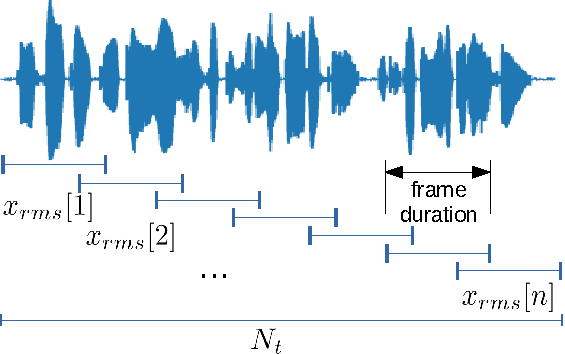
\includegraphics[width=0.8\textwidth]{../fig/silence_fig-crop.pdf}
  \caption{Silent pause features calculation}
  \label{fig:silence_fig}
\end{figure}

Figure \ref{fig:msp_threshold} shows the use of different threshold factors in
determining silent pause features. The lower threshold factor, the smaller
number of silence frames correspond to silent pause features. Thus, the choice
of silence threshold factor is also critical when calculating silent pause
features apart from the silent pause duration. Notice that leading and trailing
silences have been trimmed; hence, the calculated silent pause features are
only within the trimmed region.

\begin{figure}[htbp]
  \centering
  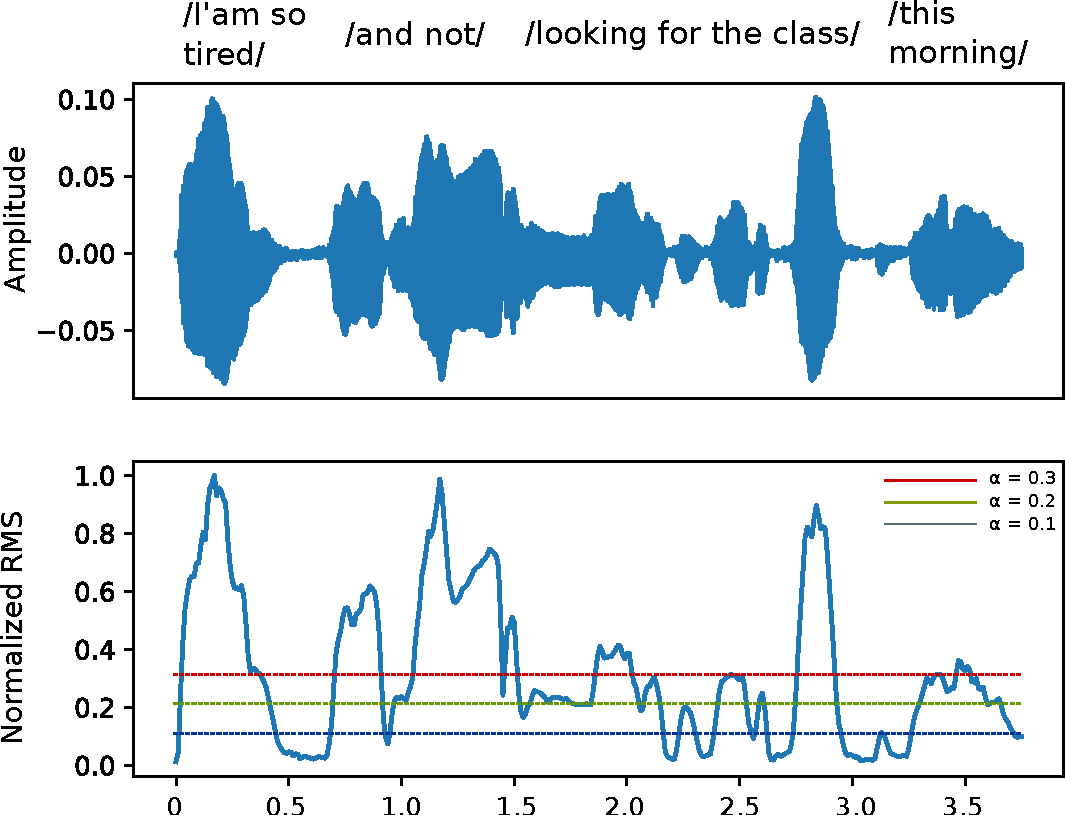
\includegraphics[width=0.8\textwidth]{../fig/msp_sa01a-trimmed.pdf}
  \caption{Different silent threshold factors on normalized RMS with 
  trimmed leading and trailing silences}
  \label{fig:msp_threshold}
\end{figure}

% todo: Algorithm for computing silent pause features (including start-end
% trimming)

% results of silence as feature
Table \ref{tab:ie_saf} and \ref{tab:msp_saf} show the result of using silence
pauses as a feature on IEMOCAP and MSP-IMPROV datasets. Both results confirm
the improvement of CCC scores from the baseline. While results on Table
\ref{tab:ie_saf} were obtained using 5 layers MLP, results on Table
\ref{tab:msp_saf} were obtained using 3 layers MLP.

Finally, Table \ref{tab:saf_recap} shows a summary of the three strategies to
observe the effect of silence on dimensional speech emotion recognition. In the
IEMOCAP dataset, utilizing silence leads to higher performance than keeping
silence. In the MSP-IMPROV dataset, removing silence leads to higher
performance than keeping silence. Both tables show the advantage of either
removing silence or utilizing silence; both lead to better performances than
the baseline score.

\begin{table}
\caption{Result of using silence as an additional feature on pAA feature set on
IEMOCAP dataset; bold-typed scores indicate a higher mean value than baseline.}
  \begin{center}
    \begin{tabular}{c | c | c c c c}
      \hline
Duration (ms)   & Threshold &  V & A & D & Mean \\
\hline \hline
10  & 0.2   & 0.273   & 0.607   & 0.424   & 0.435 \\
10  & 0.3   & 0.288   & 0.626   & 0.448   & 0.454 \\
60  & 0.1   & 0.277   & 0.606   & 0.424   & 0.436 \\
60  & 0.2   & 0.273   & 0.606   & 0.422   & 0.434 \\
60  & 0.3   & 0.283   & 0.624   & 0.447   & 0.451 \\
100 & 0.1   & 0.278   & 0.604   & 0.421   & 0.434 \\
100 & 0.2   & 0.284   & 0.624   & 0.446   & 0.451 \\
100 & 0.3   & 0.298   & 0.641   & 0.460   & \textbf{0.466} \\
      \hline
    \end{tabular}
  \end{center}
  \label{tab:ie_saf}
\end{table}

\begin{table}
\caption{Result of using silence as an additional feature on pAA feature set on
MSP-IMPROV dataset; bold-typed scores indicate a higher mean value than
baseline.}
  \begin{center}
    \begin{tabular}{c | c | c c c c}
      \hline
Duration (ms)   & Threshold &  V & A & D & Mean \\
\hline \hline
10  & 0.1   & 0.227   & 0.601   &   0.443   &   \textbf{0.424} \\
10  & 0.2   & 0.211   & 0.586   &   0.428   &   0.408 \\
10  & 0.3   & 0.209   & 0.584   &   0.427   &   0.407 \\
60  & 0.1   & 0.219   & 0.601   &   0.436   &   \textbf{0.419} \\
60  & 0.2   & 0.209   & 0.586   &   0.426   &   0.407 \\
60  & 0.3   & 0.207   & 0.585   &   0.430   &   0.407 \\
100 & 0.1   & 0.212   & 0.585   &   0.425   &   0.407 \\
100 & 0.2   & 0.208   & 0.586   &   0.430   &   0.408 \\
100 & 0.3   & 0.207   & 0.585   &   0.430   &   0.407 \\
      \hline      
    \end{tabular}
  \end{center}
  \label{tab:msp_saf}
\end{table}

% recap from all three
\begin{table}
  \caption{Comparison of three conditions for investigating the effect of silence in dimensional SER}
  \begin{center}
    \begin{tabular}{l c c c c}
      \hline
Strategy &  V & A & D & Mean \\
\hline \hline
\multicolumn{5}{c}{IEMOCAP} \\
      \hline
Removing silence  & 0.283 & 0.640 & 0.454 & 0.459 \\
Keeping silence & 0.268 & 0.641 & 0.458 & 0.456 \\
Utilizing silence & 0.298 & 0.641 & 0.460 & 0.466 \\
      \hline
\multicolumn{5}{c}{MSP-IMPROV}  \\
      \hline      
Removing silence  & 0.259 & 0.586 & 0.441 & 0.429 \\
Keeping silence & 0.217 & 0.586 & 0.425 & 0.409 \\
Utilizing silence & 0.227 & 0.601 & 0.443 & 0.424 \\
      \hline
    \end{tabular}
  \end{center}
  \label{tab:saf_recap}
\end{table}

\section{Acoustic feature aggregation}
The final issue to be discussed in this chapter is to choose which aggregation
method works best for dimensional SER from acoustic features. It is common in
audio processing to split an utterance (or story) into chunks. The goal is for
fast processing as well as for reducing the size of recorded/analyzed audio
data. While the label is only given per utterance, acoustic features extraction
is performed on chunk-based processing, either using LLDs or HSFs. Thus, two
options exist: whether aggregating input features to have single label per
utterance or aggregating outputs with many labels for a single utterance. For
the latter method, the label to represent a single story from many chunk labels
can be performed by a such method, e.g., majority voting.  

% telling acoustic features used
Seven types of LLDs from LibROSA features extractor \cite{McFee2020} were
extracted for acoustic input features: MFCCs (40 coefficients), chroma (12),
mel-spectrogram (128), spectral contrast (7), tonal centroid (6), deltas of
MFCCs (40), and deltas-deltas of MFCCs (40).  This feature set is adopted from
\cite{Atmaja2020j}. In total, there are 273 features on each frame. Following
the previous success in using global features for determining region of
analysis, Mean+Std from these 273 LLDs were extracted, resulting in
546-dimensional functional features.

% feature aggregation, % why mean and max
Input feature aggregation is a method to choose which features to represent a
set of data (story) given many recordings (chunks). Statistical functions were
widely used to aggregate many measurements. The choice of mean and maximum
values for acoustic feature aggregation is based on the assumption that
acoustic features representing emotion either from mean values (e.g., mean
intonation) or maximum values (e.g., high pitch in specific speech region when
expressing fear or happy). In maximum aggregation, the highest column vector
value of acoustic features (Mean+Std from LLDs) for each chunk on the same
stories. By using these methods, each story has the same $n$-dimensional
feature vector depends on extracted acoustic features. A similar approach was
conducted for mean values feature aggregation. Figure
\ref{fig:input_aggregation} shows acoustic input aggregation from chunks to a
story. 


% majority voting
Output aggregation is often performed by majority voting. The use of majority
voting in SER has been implemented in various techniques \cite{Sezgin2012,
Elbarougy2019, Griol2017}. The majority voting method was often used to choose
the final label over different classifiers (known as \textit{ensemble} method).
However, the majority voting defined in this study closer to its original term;
the most frequent class is chosen among other classes to represent the data. In
the INTERSPEECH 2020 elderly sub-challenge (ESC), the dataset provided audio
files as chunks, parts of an utterance/story. Acoustic features (frame-based
features and statistical functions) were extracted per this chunk and
forwarded to a classifier. Thus, in a single story, there are many labels with
regard to the number of chunks. The majority voting chooses the most frequent
label from chunks to represent a story (Figure \ref{fig:output_aggregation}).

\begin{figure}
  \centering
  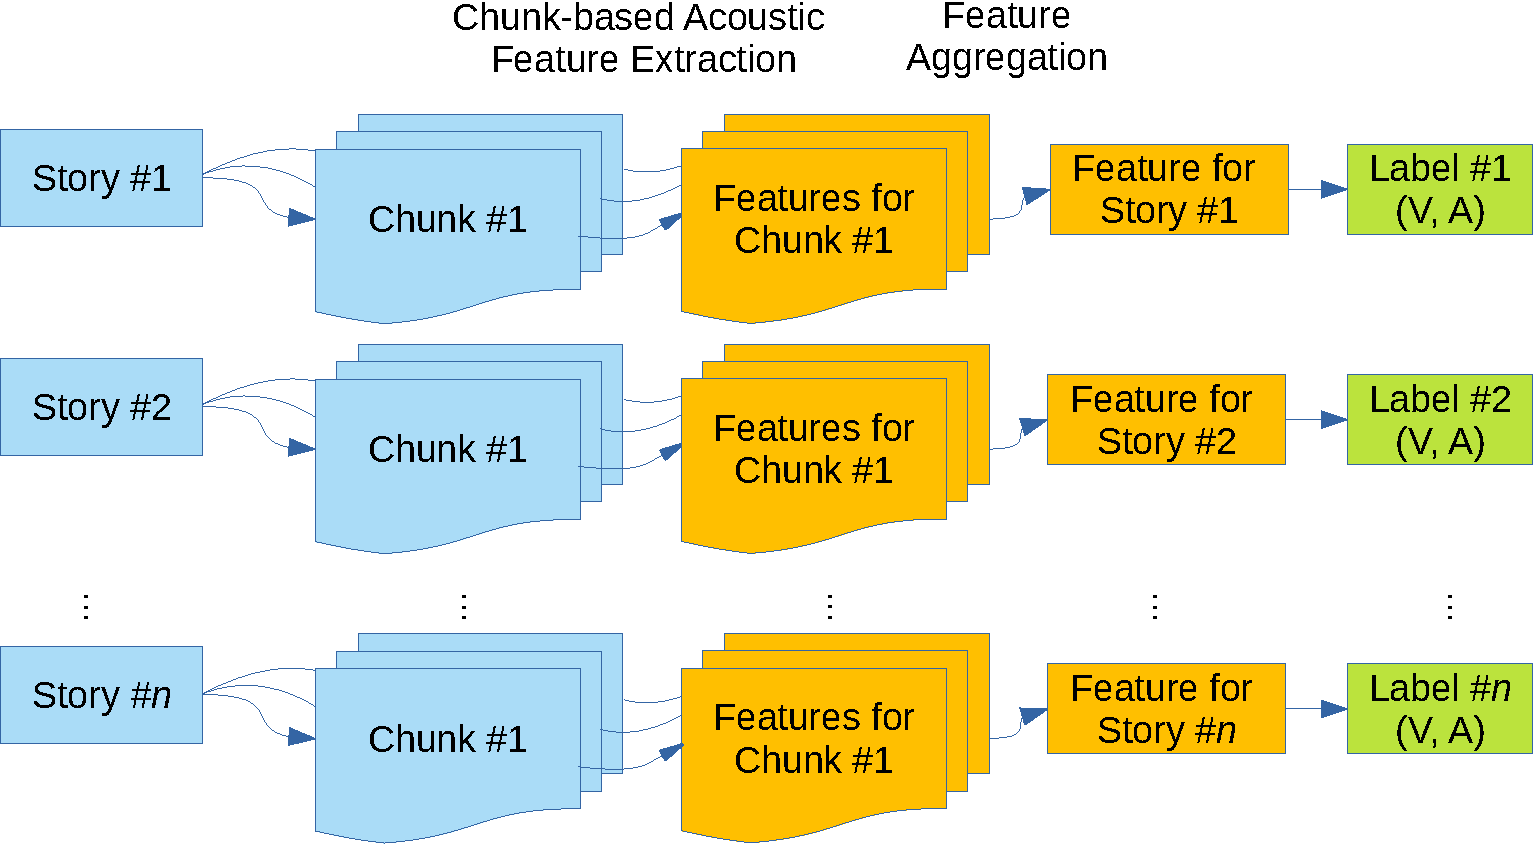
\includegraphics[width=.7\textwidth]{../fig/feature_aggregation-crop.pdf}
  \caption{Flow diagram of acoustic input feature aggregation}
  \label{fig:input_aggregation}
\end{figure}

\begin{figure}
  \centering
  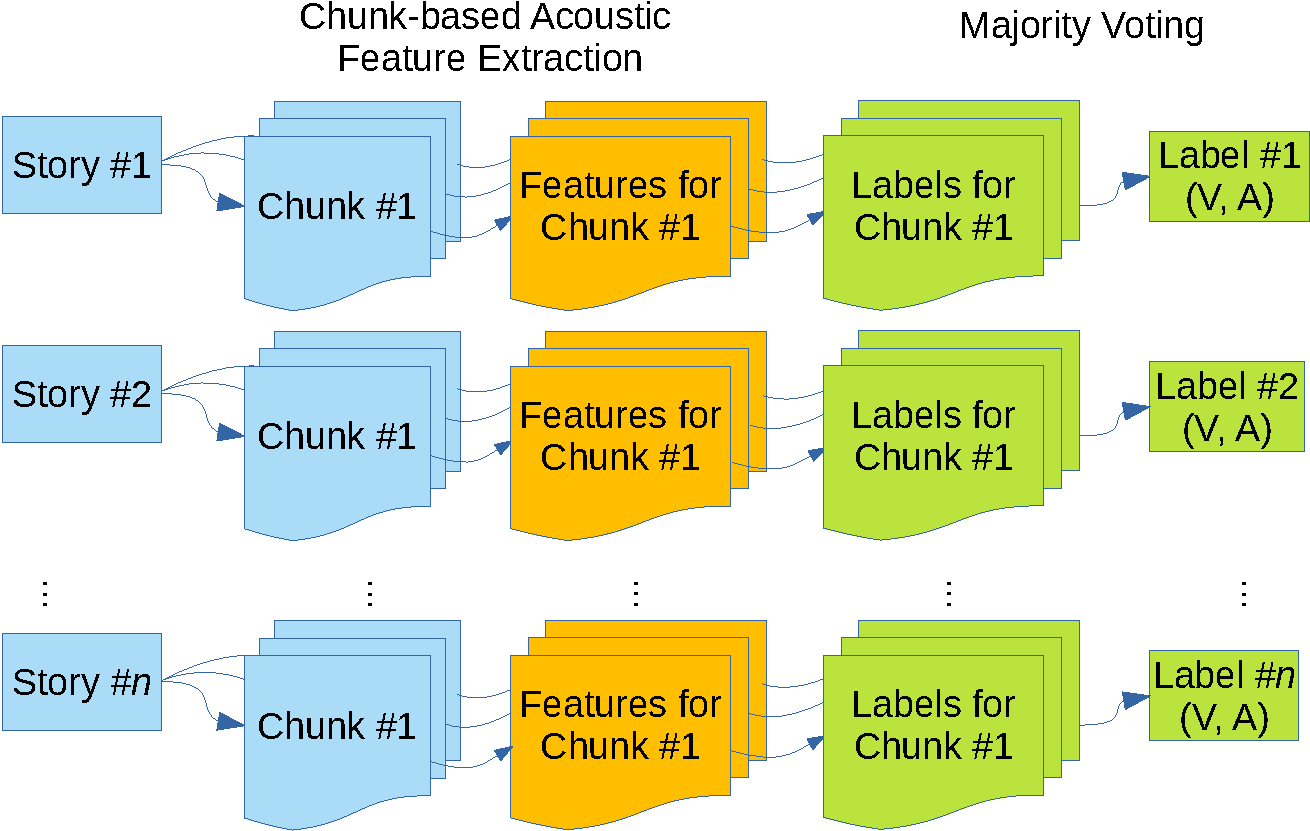
\includegraphics[width=.7\textwidth]{../fig/majority_voting-crop.pdf}
  \caption{Flow diagram of acoustic output aggregation (majority voting)}
  \label{fig:output_aggregation}
\end{figure}



% result
In comparing mean vs. maximum aggregation methods, it is found that mean
aggregation leads to higher UAR scores than maximum aggregation in development
partition. All results from mean input aggregation attain higher scores than
baseline majority voting. Table \ref{fig:input_aggregation} also shows that
mean input aggregation works better than mean output aggregation. This finding
suggests that using all chunks (by averaging) is better than choosing one value
from a chunk (by maximum value). This evidence also supports the previous
global features approach as a solution to choose the region of analysis of
acoustic features.


% Mean+Std from Compare dataset
\begin{table}
\caption{UAR results on development set: unimodal acoustic feature aggregation
vs. baseline \cite{Schuller} (INTERSPEECH 2020 ComParE Elderly Emotion
Sub-Challenge dataset)}
    \label{tab:acoustic_aggregation}
    \begin{center}
    \begin{tabular}{l c c c c c c}
    \hline 
Features  & \multicolumn{2}{c}{Majority Voting \cite{Schuller} } &
\multicolumn{2}{c}{Mean Input Agg.}      & \multicolumn{2}{c}{Max Input Agg.}
\\
& V & A & V & A & V & A \\   
\hline \hline
LibROSA Mean+Std  & - & - & \textbf{45.1}  & 38.3  & 42.7 & 39.7 \\
ComParE & 33.3  &   39.1  & 43.4  & 42.7  & \textbf{45.3} & 37.0 \\
BoAW-125  & 38.9  &   42.0& 44.6 & \textbf{45.7} & 44.6  & 40.1 \\
BoAW-250  & 33.3  & 40.5  & 43.0  & 40.8  & 39.6  & 37.6 \\
BoAW-500  & 38.9  & 41.0  & 42.6  & 41.0  & 42.9  & 37.9 \\
BoAW-1000 & 38.7  & 30.5  & 43.5  & 41.5  & 40.2  & 39.8 \\
BoAW-2000 & \textbf{40.6}  & 39.7  & 41.9  & 44.8  & 43.4  & 40.1 \\
ResNet50  & 31.6  & 35.0  & 36.5  & 36.7  & 37.1  & 39.0 \\
AuDeep-30 & 35.4  & 36.2  & 38.4  & 42.1  & 42.8  & 35.6 \\
AuDeep-45 & 36.7  & 34.9  & 39.5  & 40.5  & 39.3  & 33.3 \\
AuDeep-60 & 35.1  & \textbf{41.6}  & 43.4  & 42.1  & 40.7  & 41.4 \\
AuDeep-75 & 32.7  & 40.4  & 41.9  & 44.4  & 40.9  & \textbf{43.3} \\
AuDeep-fused  & 29.2  & 36.3  & 43.6  & 39.5  & 42.2  & 39.3 \\
    \hline
    \end{tabular}
  \end{center}
  \end{table}

% why not use features from all chunks, i.e., without any aggregation method
The use of aggregation methods reduces feature dimension (for input to
classifier) and computational complexity. Using all chunks to process the data,
e.g., without feature aggregation, increase computational load and complexity.
The number of samples became larger according to the number of chunks. However,
the UAR score is low. Using feature aggregation not only reduces complexity and
feature dimension but also increases the performance score.

Although this evaluation of the aggregation method for speech emotion
recognition is not intended to mimic human auditory perception, there may be a
similarity in human auditory perception on aggregating different cues. Humans
may use the aggregation of prosodic information from short-term voices for
longer-time emotion perception. The initial goal of this feature aggregation
is, indeed, to concatenate acoustic features with linguistic features, which
will be explained in the next chapter. 

% The content following two sections can be included in summary and previous
% sections \section{Effect of Different Acoustic Features} \section{Effect of
% Different Classifiers}
\section{Summary}
This chapter presents an evaluation of speech emotion recognition from acoustic
information. Three problems are investigated, including the region of analysis
for feature extraction, the silent pause region's effect, and the aggregation
methods. Table \ref{tab:sum_ch4} presents the results of these investigations.
On the first problem, it was found consistently that high-level statistical
functions obtained better performance than low-level descriptors.  This result
shows that small-feature size is not a problem for DNN-based classifiers
(instead, the number of data still a problem). Mean and standard deviation from
acoustic features showed meaningful representation for acoustic-based emotion
recognition. The second evaluation of the silent pause region's effect showed
that either removing silence or utilizing silence as a feature leads to a
better performance than using acoustic features from the whole speech region.
Between the two, it is difficult to choose which one is better based on the
current results. The results predict the important role of silent in emotion.
The third evaluation showed that the input aggregation method showed better
performances than output aggregation by majority voting. Not only improving the
performance, this aggregation technique made the ability for concatenating
acoustic features with other features. While the first two issues are the major
issues in SER research, the finding on the third issue needs generalization and
confirmation in other datasets and scenarios.

The use of only acoustic features in this study still shows some lacks in
dimensional SER; the major drawback is the low performance of valence
prediction. This drawback of acoustic-based SER leads to the investigation of
fusing acoustic information with other modalities. The next chapter presents
fusion of acoustic with linguistic information at feature level. 

\begin{table}[htbp]
  \caption{Summary of study on dimensional SER using acoustic features}
  \begin{center}
  \begin{tabular}{l| ccc}
  \hline
Issue & \multicolumn{3}{c} {Proposed method} \\
\hline \hline
Region of analysis  & \mybox{frames} & & utterance (fixed length) \\
Silence region   & removing silence  & \mybox{keeping silence} & utilizing
silence\\
Aggregation method  & input aggregation & & \mybox{output aggregation} \\
  \hline
  \end{tabular}
  \label{tab:sum_ch4}
\end{center}
\end{table}


% \newpage
% \thispagestyle{empty}
% \mbox{}
